% Dokoumentenklassen legen das grobe Layout fest. Hier wird eine selbsterstellte Klasse verwendet, deswegen benötigt man zum erstellen des PDFs auch die Datei uebungsblatt.cls und uebungsblatt.sty
\documentclass{uebungsblatt}

\usepackage[linesnumbered,commentsnumbered]{algorithm2e}
\usepackage{tikz}
\usepackage{hyperref}
% Store \nl in \oldnl
\let\oldnl\nl
% Remove line number for one line
\newcommand{\nonl}{\renewcommand{\nl}{\let\nl\oldnl}}

%Hier wird die Kopfzeile erstellt
\header{\textbf{Grundlagen der Praktischen Informatik}\hfill\textbf{Sommersemester 2024}\\
Student:in1 (Matrikelnummer1) % Name des Gruppenmitglieds Eintragen
\hfill Georg-August-Universität Göttingen \\
Student:in2 (Matrikelnummer2)  % Name des Gruppenmitglieds Eintragen
\hfill Institut für Informatik\\ 
Student:in3 (Matrikelnummer2)\\  % Name des Gruppenmitglieds Eintragen
Student:in4 (Matrikelnummer2)\\  % Name des Gruppenmitglieds Eintragen

% Hiermit wird der horizontale Strick erzeugt, der die Kopfzeile abgrenzt.
\rule{\textwidth}{0.1mm}}

% Hier wird die Blattnummer festgelegt.
\blattnummer{4}

% Hier beginnt der eigentliche Textkörper. Alles zwischen \begin{document} und \end{document} ist der eigentliche Text
\begin{document}

% Mit \underline kann man Sachen unterstreichen


% \begin{aufgabe} erstellt ein Aufgabenumgebung mit [...] könnt ihr den Titel angeben und mit \score die Punktzahl festlegen. Ist aber für euch nicht so wichtig.
\begin{aufgabe}[Reguläre Sprachen \score{17}]
Sei $L$ die Sprache aller Wörter $w \in \{0,1,\ldots,9\}^*$ für die gilt, dass die Ziffernfolge $w$, interpretiert als
ganze Zahl, ohne Rest durch 3 teilbar ist. 
Besteht die Ziffernfolge $w$ aus mehr als einer Ziffer, muss die erste Ziffer ungleich 0 sein.
Das leere Wort ist nicht in der Sprache enthalten. 

\smallskip
Ist die Sprache $L$ regulär?

\smallskip
\underline{Hinweis:}
Ein Zahl ist ohne Rest durch 3 teilbar, wenn die
Quersumme ohne Rest durch 3 teilbar ist.\\
\score{17}

\end{aufgabe}
% Hier könnt ihr eure Lösung hinschreiben
\begin{loesung} 

\end{loesung}
\newpage
%-----------------------------
\begin{aufgabe}[Äquivalente Automaten \score{20}]
Geben Sie zu dem nachfolgend abgebildeten Zustandsgraphen eines
nichtdeterministischen endlichen Automaten über dem Alphabet $\Sigma = \{a,b\}$ 
einen äquivalenten (vollständigen) deterministischen endlichen Automaten an.\\
\begin{center}
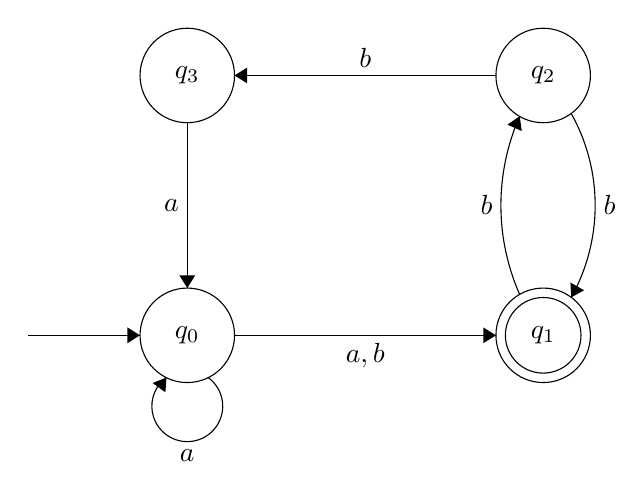
\begin{tikzpicture}[scale=0.2]
\tikzstyle{every node}+=[inner sep=0pt]
\draw [black] (14.2,-36.9) circle (3);
\draw (14.2,-36.9) node {$q_0$};
\draw [black] (14.2,-20.4) circle (3);
\draw (14.2,-20.4) node {$q_3$};
\draw [black] (36.8,-20.4) circle (3);
\draw (36.8,-20.4) node {$q_2$};
\draw [black] (36.8,-36.9) circle (3);
\draw (36.8,-36.9) node {$q_1$};
\draw [black] (36.8,-36.9) circle (2.4);
\draw [black] (4.1,-36.9) -- (11.2,-36.9);
\fill [black] (11.2,-36.9) -- (10.4,-36.4) -- (10.4,-37.4);
\draw [black] (14.2,-23.4) -- (14.2,-33.9);
\fill [black] (14.2,-33.9) -- (14.7,-33.1) -- (13.7,-33.1);
\draw (13.7,-28.65) node [left] {$a$};
\draw [black] (33.8,-20.4) -- (17.2,-20.4);
\fill [black] (17.2,-20.4) -- (18,-20.9) -- (18,-19.9);
\draw (25.5,-19.9) node [above] {$b$};
\draw [black] (17.2,-36.9) -- (33.8,-36.9);
\fill [black] (33.8,-36.9) -- (33,-36.4) -- (33,-37.4);
\draw (25.5,-37.4) node [below] {$a,b$};
\draw [black] (35.306,-34.305) arc (-156.19851:-203.80149:14.013);
\fill [black] (35.31,-22.99) -- (34.53,-23.52) -- (35.44,-23.93);
\draw (33.61,-28.65) node [left] {$b$};
\draw [black] (38.577,-22.808) arc (29.24158:-29.24158:11.96);
\fill [black] (38.58,-34.49) -- (39.4,-34.04) -- (38.53,-33.55);
\draw (40.6,-28.65) node [right] {$b$};
\draw [black] (15.523,-39.58) arc (54:-234:2.25);
\draw (14.2,-44.15) node [below] {$a$};
\fill [black] (12.88,-39.58) -- (12,-39.93) -- (12.81,-40.52);
\end{tikzpicture}
\end{center}
\medskip
\underline{Hinweise:} 
\begin{itemize}
    \item Sie können den Automaten entweder durch einen Zustandsgraphen darstellen oder über eine Tabelle mit der Übergangsfunktion. Wollen Sie einen Zustandsgraphen erstellen, können sie folgende Seite verwenden: \href{https://madebyevan.com/fsm/}{Finite State Machine Designer}. Dort können Sie sich ebenfalls direkt \LaTeX \ Code für den Automaten generieren lassen. 
    \item Bei einem (vollständigen) deterministischen endlichen Automaten ist für jeden Zustand für alle Zeichen des Alphabets ein nachfolgender Zustand definiert.
\end{itemize}



\smallskip
\score{20}
\end{aufgabe}
\begin{loesung}
Beispiel mit Tabelle:\\
$A = (\Sigma, Q, s, F, \delta)$
\begin{itemize}
    \item Alphabet $Sigma = \{a,b\}$ 
    \item Zustände $Q = \{\{q_0\}, \dots \}$
    \item Startzustand $s = \{q_0\}$
    \item Akzeptierende Zustände $F = \{ \dots \}$
    \item Überführungsfunktion $delta : Q \times Sigma \rightarrow Q$
\end{itemize}

\smallskip
\underline{Hinweis:}
Die Zustandsmenge sowie die Endzustände müssen noch ergänzt werden. Ebenfalls muss die unterstehende Tabelle für die Übergangsfunktion ergänzt werden.

\begin{center}
%Hier ist der Text links bündig (l = left)
    \begin{tabular}{l|l|l}
    $p \in Q$ & $\delta_p(a)$ & $\delta_p(b)$ \\
    \hline
    $\{q_0\}$ & $\{q_0, q_1\}$ & $\{q_1\}$      \\
    $\{q_1\}$ &  &  \\
    $\{q_2\}$ &  &  \\
    $\{q_3\}$ &  &  \\
    $\{q_0, q_1\}$ &  &  \\
    $\{q_0, q_2\}$ &  &  \\
    \end{tabular}
\end{center}
\end{loesung}
\newpage
\begin{aufgabe}[Operationen auf Regulären Sprachen \score{25}]
\underline{Behauptung.}

\smallskip
Sind $L_1, L_2$ reguläre Sprachen, dann ist auch der Durchschnitt  der beiden Sprachen regulär.
\begin{align*}
L_1 \cap L_2:=\{w \mid w\in L_1\text{ und }w\in L_2\}    
\end{align*}
Seien $A_1 = (\Sigma_1, Q_1, q_1, F_1, \delta_1)$ und $A_2 = (\Sigma_2, Q_2, q_2, F_2, \delta_2)$ 
deterministische endliche Automaten, für die gilt $A_1$ akzeptiert $L_1$
und $A_2$ akzeptiert $L_2$.

\medskip
Zeigen Sie die Behauptung, indem Sie aus $A_1$ und $A_2$ einen
deterministischen endlichen Automaten konstruieren, der $L_1 \cap L_2$ akzeptiert.\\
\score{25}

\end{aufgabe}
% Hier könnt ihr eure Lösung hinschreiben
\begin{loesung}

\end{loesung}
\end{document}
